\pdfminorversion=4 % for acroread
\documentclass[t]{beamer}
%\documentclass[t,handout]{beamer}

\usepackage[english]{babel}
\usepackage[utf8]{inputenc}
\usepackage{graphicx}

\usepackage{amsmath,amssymb}
\usepackage{listings}
\lstset{frame=lines,framesep=3pt,numbers=left,numberblanklines=false,basicstyle=\ttfamily\small}

\usepackage{subfig}
\usepackage{multicol}
\usepackage{appendixnumberbeamer}

\usepackage{tikz}
\usetikzlibrary{trees} 
\usetikzlibrary{shapes.geometric}
\usetikzlibrary{positioning,shapes,shadows,arrows,calc,mindmap}
\pgfdeclarelayer{background}
\pgfdeclarelayer{foreground}
\pgfsetlayers{background,main,foreground}
\tikzstyle{activity}=[rectangle, draw=white, rounded corners, text centered, text width=8em]
\tikzstyle{data}=[rectangle, draw=white, text centered, text width=8em]
\tikzstyle{myarrow}=[->, thick, draw=white]

% Define the layers to draw the diagram
\pgfdeclarelayer{background}
\pgfdeclarelayer{foreground}
\pgfsetlayers{background,main,foreground}


\usepackage{listings}
\lstset{numbers=left,
  showstringspaces=false,
  frame={tb},
  captionpos=b,
  lineskip=0pt,
  basicstyle=\ttfamily,
  extendedchars=true,
  stepnumber=1,
  numberstyle=\small,
  xleftmargin=1em,
  breaklines
}

 

\usetheme{Madrid}
\useinnertheme{rectangles}
\usecolortheme{whale}
\setbeamercolor{alerted text}{fg=blue}
\useoutertheme{infolines}
\setbeamertemplate{navigation symbols}{\vspace{-5pt}} % to lower the logo
\setbeamercovered{invisible}

\makeatletter
\setbeamertemplate{footline}
{
  \leavevmode%
  \hbox{%
  \begin{beamercolorbox}[wd=.333333\paperwidth,ht=2.25ex,dp=1ex,center]{author in head/foot}%
    \usebeamerfont{author in head/foot}\insertshortauthor
  \end{beamercolorbox}%
  \begin{beamercolorbox}[wd=.333333\paperwidth,ht=2.25ex,dp=1ex,center]{title in head/foot}%
    \usebeamerfont{title in head/foot}\insertshorttitle
  \end{beamercolorbox}%
  \begin{beamercolorbox}[wd=.333333\paperwidth,ht=2.25ex,dp=1ex,right]{date in head/foot}%
    \usebeamerfont{date in head/foot}\insertshortdate{}\hspace*{2em}
    \insertframenumber\hspace*{2ex} 
  \end{beamercolorbox}}%
  \vskip0pt%
}
\makeatother

\newcommand{\lit}[1]{{\footnotesize\color{black!70}[#1]}}
\newcommand{\litw}[1]{{\footnotesize\color{black!20}[#1]}}

\pgfdeclareimage[height=1.2cm]{coseallogo}{images/logos/coseal}
\pgfdeclareimage[height=1.2cm]{mlaad}{images/logos/ml4aad.png}
\pgfdeclareimage[height=1.2cm]{freiburg}{images/logos/freiburg}

\logo{\pgfuseimage{freiburg}}

\title[MLOAD]{Machine Learning and Optimization\\ for Algorithm Design}
\subtitle{Feedback on Exercise 5}
\author{Marius Lindauer}
\institute{University of Freiburg}
\date{}
%\date{LION 2015, Lille, France}

% \AtBeginSection[] % Do nothing for \section*
% {
%   \begin{frame}{Outline}
%     \bigskip
%     \vfill
%     \tableofcontents[currentsection]
%   \end{frame}
% }


\begin{document}

% ----------------------------------------------------------------------
{
\setbeamertemplate{footline}{} % remove footer on first slide
	\frame[c]{
	\titlepage
	\begin{center}
	\vspace{-1.5cm}
	%
\includegraphics[height=5em]{images/logos/freiburg}\quad\quad
	%
\includegraphics[height=5em]{logo/coseal}\quad
	
\includegraphics[height=5em]{images/logos/ml4aad.png}
	\end{center}
	}
}
\author{Lindauer}
\institute{}
%\logo{\pgfuseimage{mlaad}}
\logo{}

%----------------------------------------------------------------------------------
%----------------------------------------------------------------------------------
\begin{frame}[c,fragile]{Exercise 1}

\centering
$\mathrm{E}(\bar{x}) =  \mathrm{E}(\frac{1}{n} \sum_{i=1}^n x_i) = \frac{1}{n} \sum_{i=1}^n \mathrm{E}(x_i) = \frac{1}{n} \cdot n \cdot \mu = \mu$\\
\medskip
$\to \mu_{\bar{x}} = \mu$

\bigskip
\vspace{2em}
\pause

$Var(\bar{x}) = Var(\frac{1}{n} \sum_{i=1}^{n} x_i)$\\[1em]
 
$= \frac{1}{n^2} Var(\sum_{i=1}^{n} x_i)$\\[1em]

$= \frac{1}{n^2} \sum_{i=1}^{n} Var(x_i)$\\[1em]
 
$= \frac{1}{n^2} \sum_{i=1}^{n} \sigma^2 = \frac{\sigma^2}{n}$\\[1em]

$\to \sigma^2_{\bar{x}} = \frac{\sigma^2}{n}$

\end{frame}
%----------------------------------------------------------------------------------
%----------------------------------------------------------------------------------
\begin{frame}[c,fragile]{Exercise 2: Feedback}

\begin{itemize}
  \item Add labels on x-axis and y-axis.
  \medskip
  \item To compare two configurations, they should be shown in the same plot.
  \medskip
  \item Do not completely retrain the random forest for each new number iterations.
  \medskip
  \item Use the same colors in all plots.
  \medskip
  \item Empirical CDFs are step functions.
\end{itemize}

\end{frame}
%----------------------------------------------------------------------------------
%----------------------------------------------------------------------------------
\begin{frame}[c,fragile]{Exercise 2: Performance on Test}

\centering
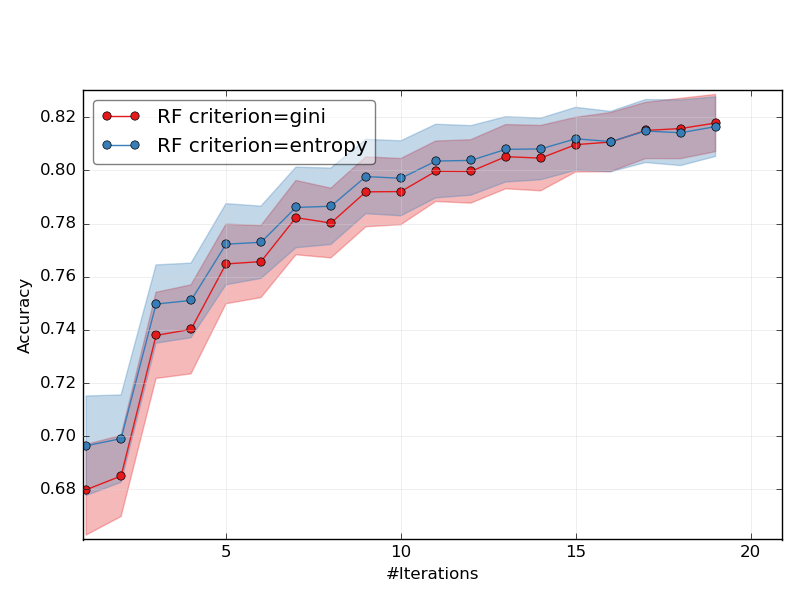
\includegraphics[width=0.8\textwidth]{rf_plots/test_mean_comparison}

\end{frame}
%----------------------------------------------------------------------------------
%----------------------------------------------------------------------------------
\begin{frame}[c,fragile]{Exercise 2: RDF at acc=0.76}

\centering
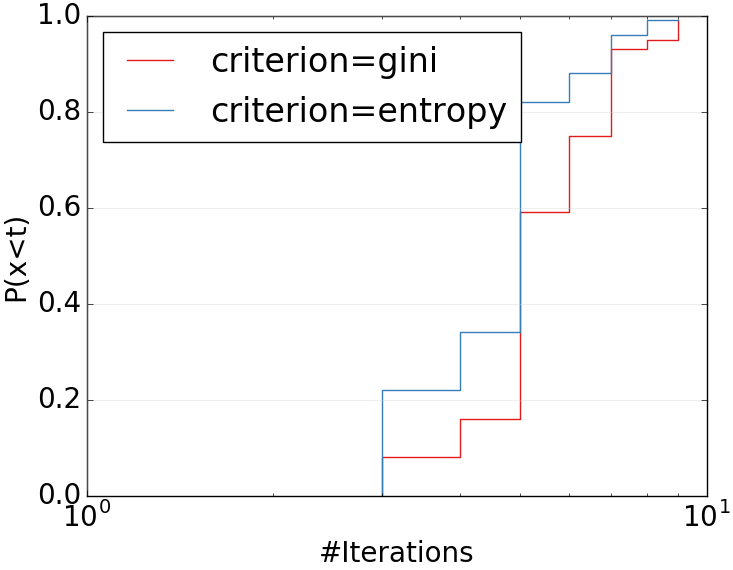
\includegraphics[width=.6\textwidth]{rf_plots/gini_entropy_cdf}

\end{frame}
%----------------------------------------------------------------------------------
%----------------------------------------------------------------------------------
\begin{frame}[c,fragile]{Exercise 3: Feedback}

\begin{itemize}
  \item Use log-scale on y-axis in box-plots (if appropriate).
  \medskip
  \item Something is wrong if all points are on the diagonal in a scatter plot.
  \medskip
  \item Use a paired permutation test when you have instances.
\end{itemize}

\end{frame}
%----------------------------------------------------------------------------------
%----------------------------------------------------------------------------------
\begin{frame}[c,fragile]{Score Overview}

\centering
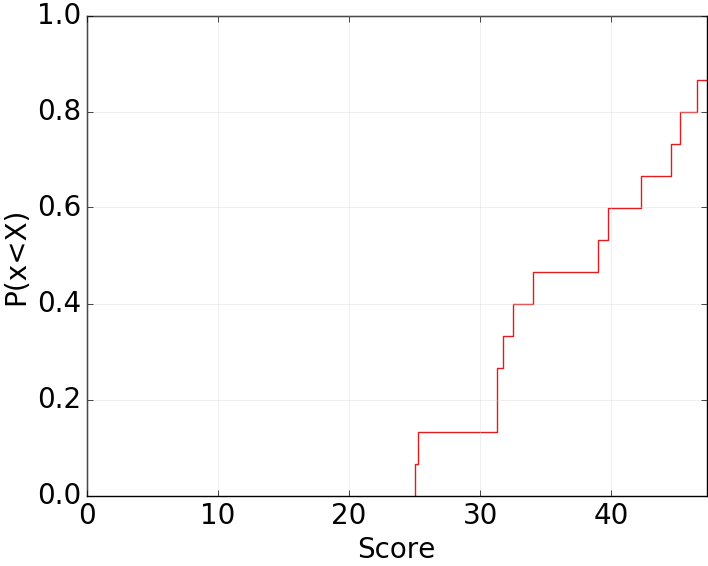
\includegraphics[width=0.8\textwidth]{scores_cdf.png}

\end{frame}
%----------------------------------------------------------------------------------
%----------------------------------------------------------------------------------
% \begin{frame}[c,fragile]{t}
% l
% \end{frame}
% %----------------------------------------------------------------------------------
% %----------------------------------------------------------------------------------
% \begin{frame}[c,fragile]{t}
% l
% \end{frame}
%----------------------------------------------------------------------------------
%----------------------------------------------------------------------------------

\end{document}
